\section{System Overview}
The FPGA Oscilloscope \textsuperscript{\textregistered} is designed to mimic some of the more used functions of a traditional digital oscilloscope, but in a much smaller package. It has two analog inputs, an 8-bit logic analyzer, hardware buttons and rotary encoders, and a 480x272 RGB display.

\begin{figure}[ht!]
    \centering
    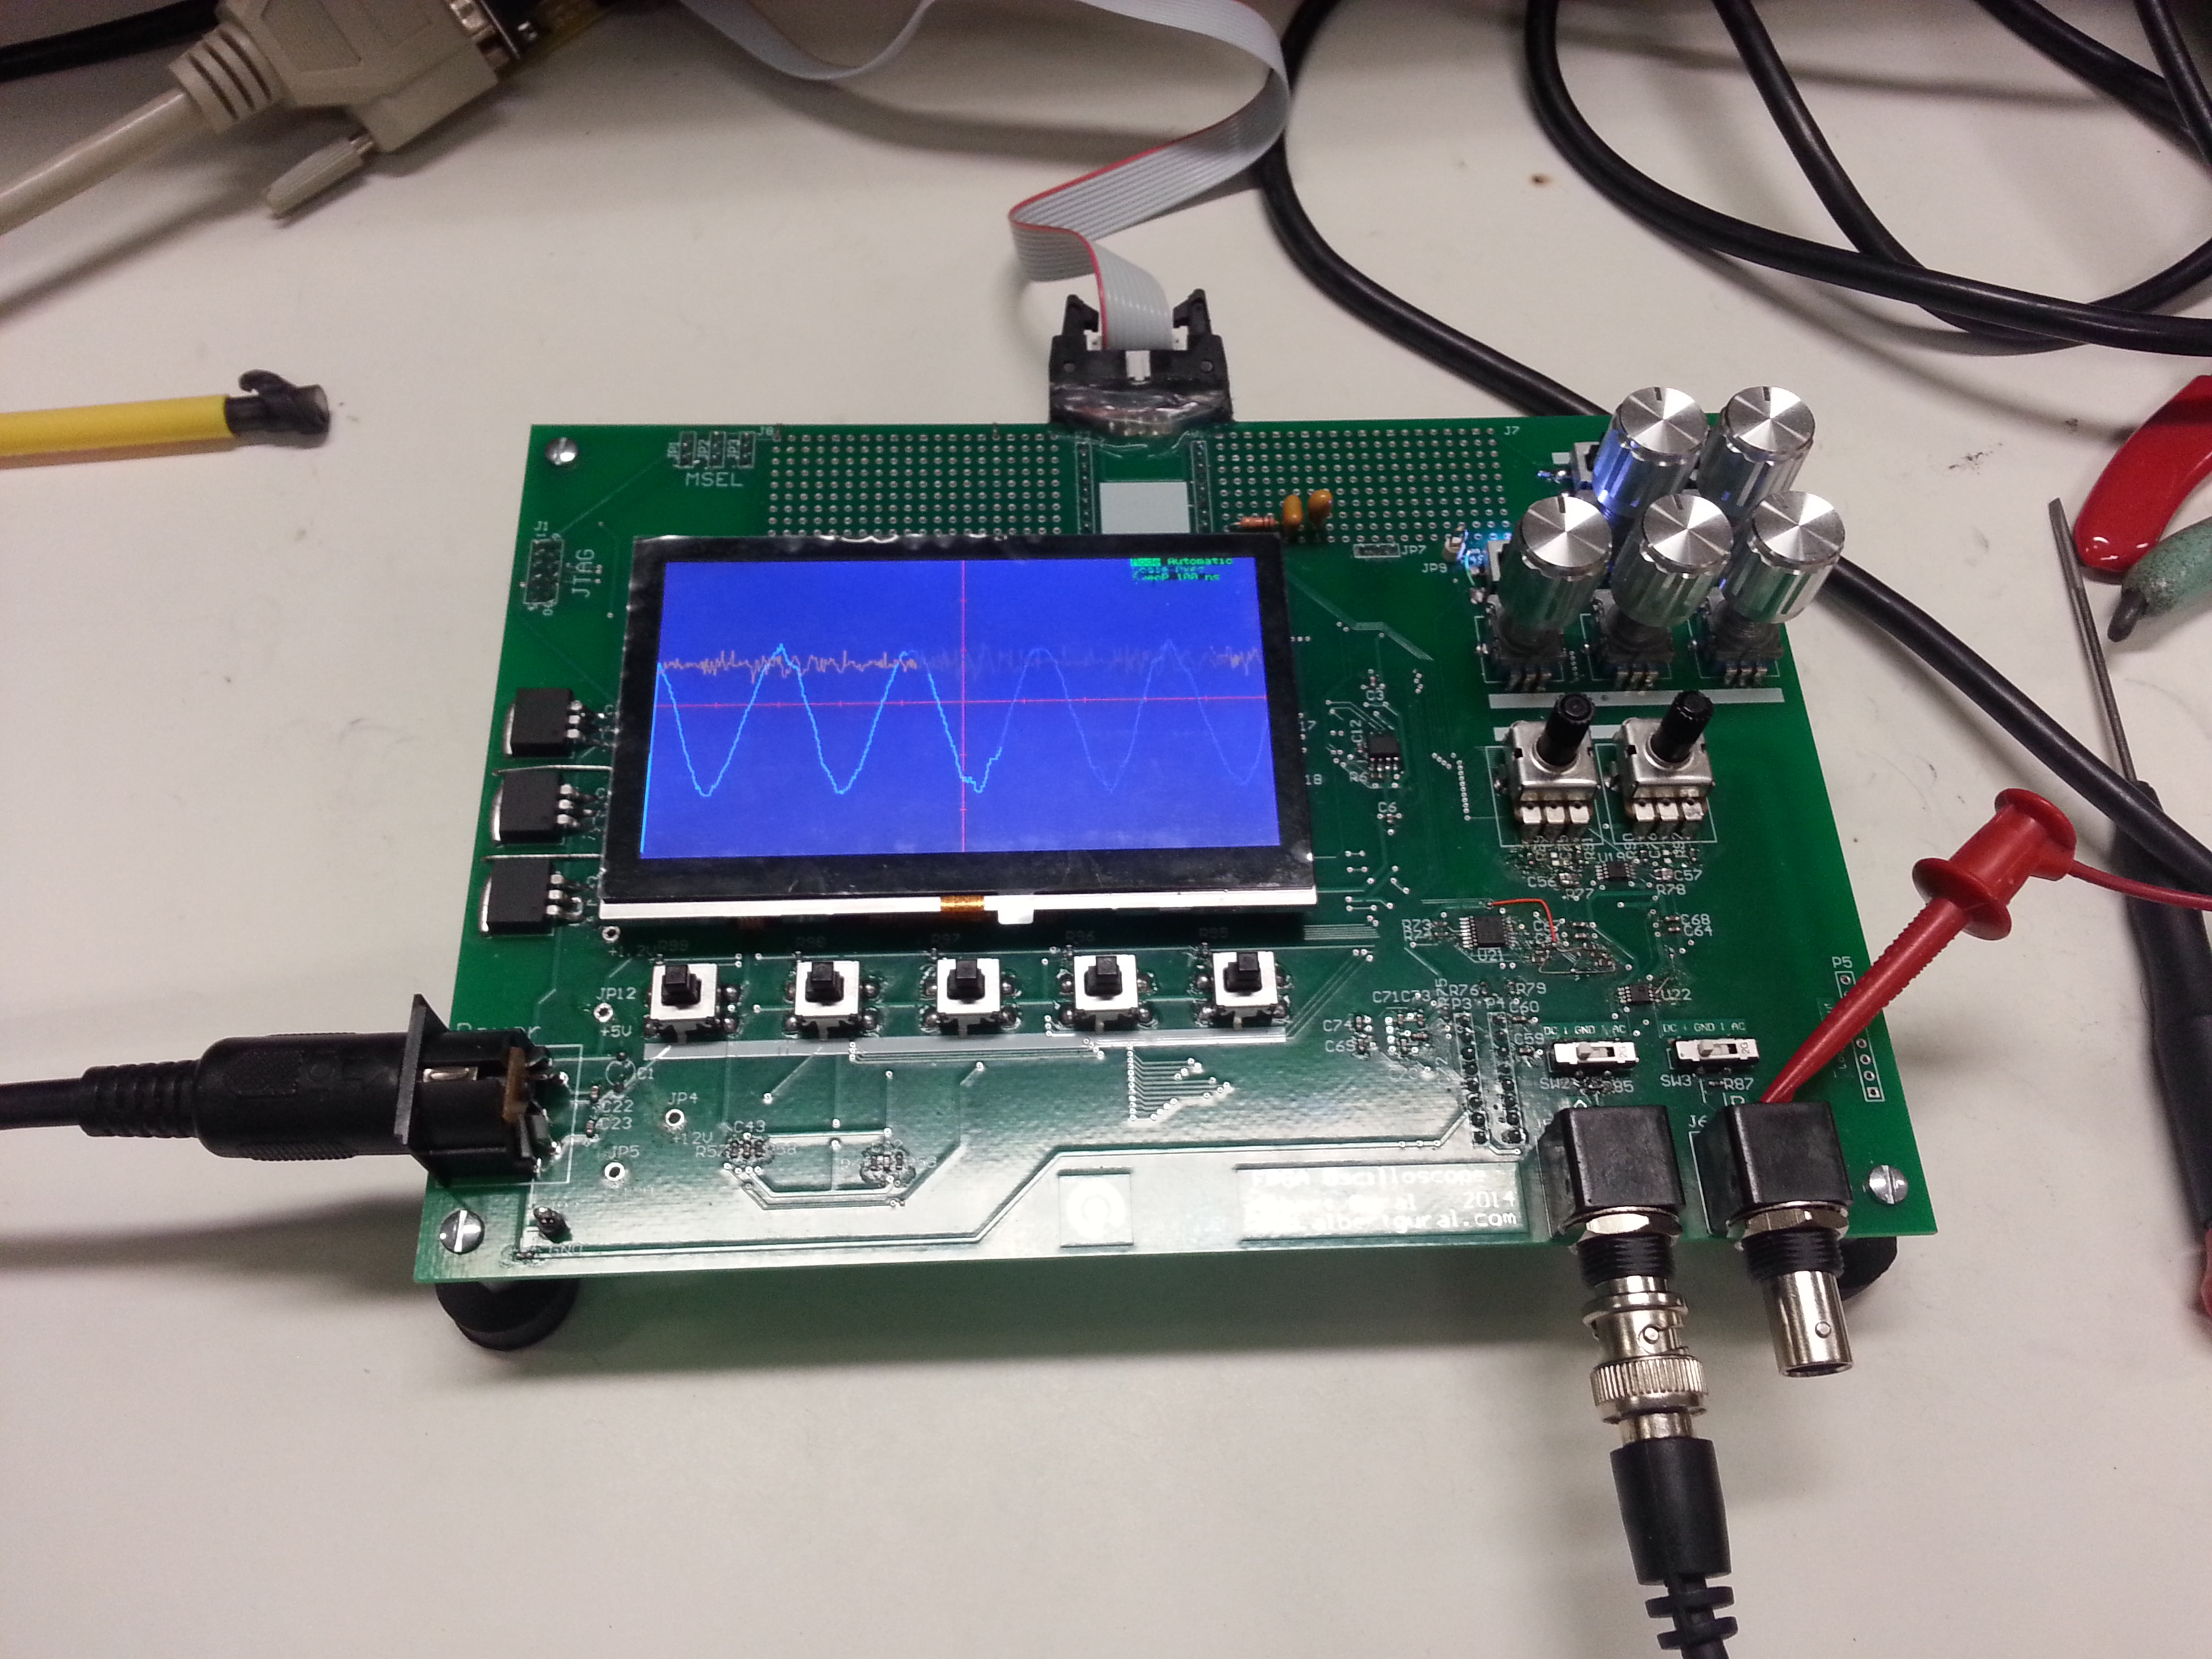
\includegraphics[width=6in]{images/osc_full.jpg}
		\caption{FPGA Oscilloscope}
\end{figure}

The system includes the main oscilloscope board (seen above), the power adapter (which supplies $5V$ and $\pm 12V$), a USB JTAG programmer, and two $1x$/$10x$ analog probes.

\section{Setup}
This version of the oscilloscope does not come pre-configured with program memory in flash, although the FPGA configuration information is programmed onto a serial flash chip. The set of operations to get the system up and running is thus:

\begin{enumerate}
	\item Install Quartus web edition (free). Download the program files from \url{https://github.com/agural/FPGA-Oscilloscope}.
	\item Plug in power to the oscilloscope. Connect the USB JTAG connector between the computer and the oscilloscope.
	\item Open up the ``NIOS II Software Build Tools for Eclipse''.
	\item Go to \verb|File > New > NIOS II Application and BSP from Template|.
	\item Select the SOPC file from \verb|<FPGA Download Directory>/osc|. Name the project whatever you want, and select ``Blank Template''.
	\item Copy code from \verb|<FPGA Download Directory>/osc/software/osc| to your Eclipse project.
	\item Compile and download the code to the oscilloscope.
\end{enumerate}

At this point, the oscilloscope should be running. Try connecting a $0.5V$ amplitude sine wave at $100kHz$ to the scope.

\section{Interface}

User control is broken into two main input methods that are mostly redundant with each other (select whichever you prefer): oscilloscope mimic controls and on-screen menu controls.

\subsection{On-screen Menu}
This menu can be used to control all software-controllable aspects of the oscilloscope and is controlled via the five hardware buttons located below the display. The menu appears on the top-right of the display. The left-most button is the menu button. Pressing this toggles the menu on and off. From left to right, the remaining buttons are ``Up'', ``Down'', ``Left'', and ``Right''. Press ``Up'' or ``Down'' to select a menu item (the selected item will be highlighted). For a given menu item, you can change its value by pressing ``Left'' or ``Right''. For example, hitting the ``Down'' button to get delay, then hitting the ``Right'' button will increase the (positive) delay by a single sample. Pressing and holding the buttons will cause them to auto-repeat.

Here are the menu items and values you can choose from:
\begin{itemize}
	\item Mode
		\begin{itemize}
			\item Auto triggering - triggers if it can, or if not, displays the sample after a given timeout.
			\item Normal triggering - updates the display only on triggers.
			\item One-shot - triggers only once and holds that on the display.
		\end{itemize}
	\item Scale
		\begin{itemize}
			\item Scale Axes - Displays just the x-y axes with tick marks at the major divisions.
			\item Scale Grid - Displays a grid of the major divisions.
			\item None - Displays only the traces (and possibly the menu).
		\end{itemize}
	\item Sweep - Sets the time per sample for the oscilloscope. Cycles through the available sweep rates (see \ref{techspecs} for a list).
	\item Trigger - Re-arms the one-shot trigger when ``Left'' or ``Right'' is pressed.
	\item Level - Sets the trigger level. It is set up to display a voltage, but this is inaccurate.
	\item Slope - Either ``Left'' or ``Right'' will toggle positive to negative slope.
	\item Delay - Sets the trigger delay. It can be changed from $-480$ to $50,000$ samples, in the appropriate time units.
\end{itemize}

\subsection{Oscilloscope-mimic Controls}
There are two latching pushbutton switches in the top-right of the oscilloscope, two rotary encoders directly below them, and three rotary encoders below these. Below that is two potentiometers, and finally two 3-position slide switches. Since the operation of these is the same as for the menu, the image below should be sufficient.

\begin{figure}[ht!]
    \centering
    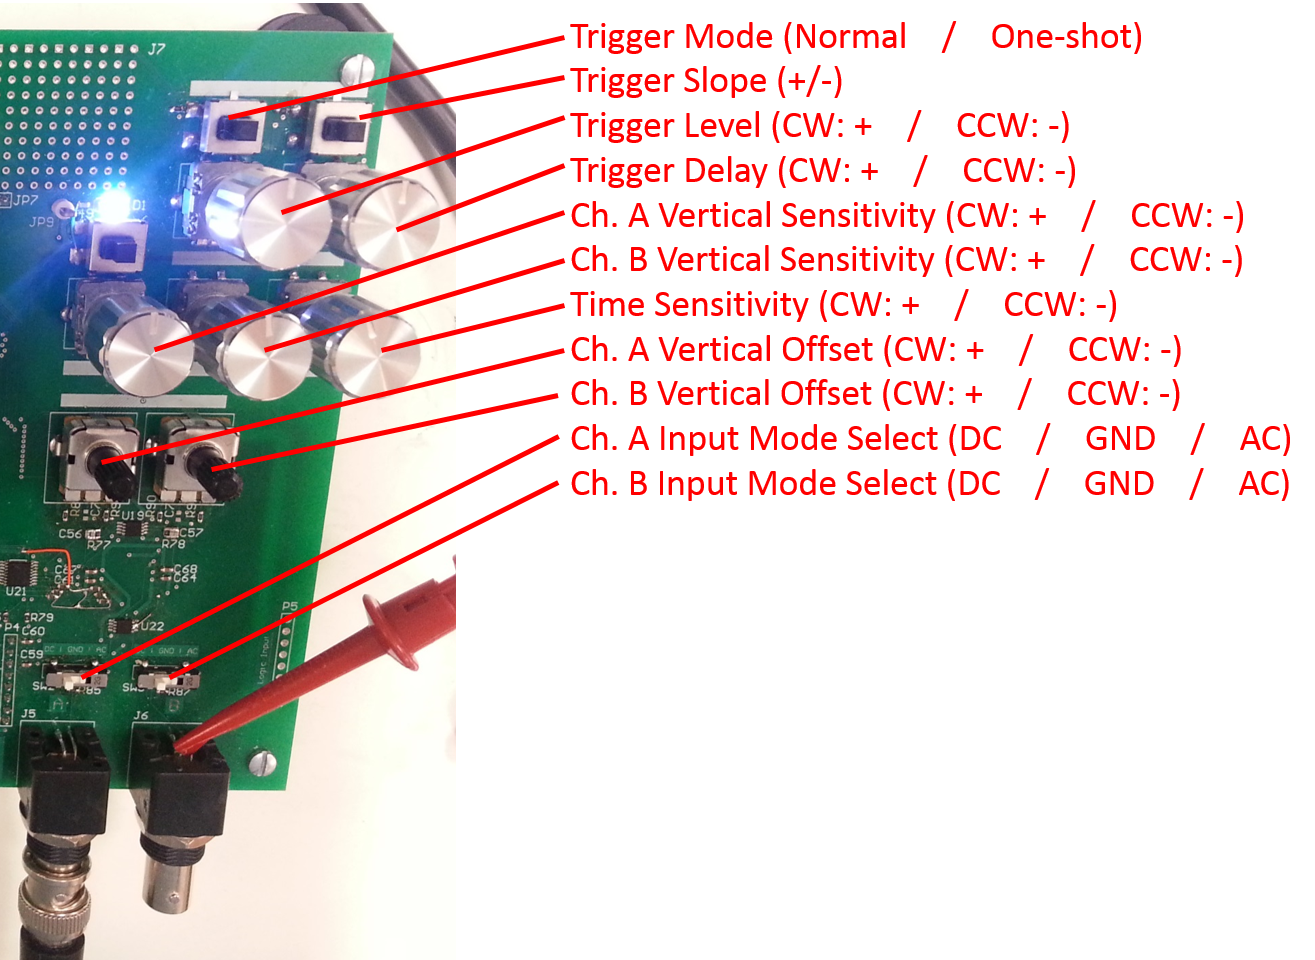
\includegraphics[width=3in]{images/hardware_buttons.png}
		\caption{Hardware buttons}
\end{figure}

The potentiometers and slide switches are the only items not do-able by the menu method (they are part of the analog frontend). Vertical sensitivity has not been completed in terms of software, although all the supporting hardware is there. All other functions follow exactly as in the case of the menu.

\section{Technical Specifications}\label{techspecs}
\subsection{Physical Specifications}
\begin{itemize}
	\item Processor: NIOS II softcore processor at $36MHz$ on an Altera Cyclone III EP3C25 (240 pin QFP) chip.
	\item RAM: 64KB x 8bit accessible SRAM.
	\item ROM: 64KB x 8bit accessible Flash.
	\item Display: 480x272 RGB display with 24-bit color (only 15-bit hardware-accessible). Also includes a 10-point capacitive touch pad overlay (hardware accessible, but not used in firm/software).
	\item Buttons: (5) screen menu buttons (momentary), (2) trigger option buttons (latching), (5) rotary encoders, (1) reset button (momentary).
	\item Ports: $5V$ and $\pm 12V$ power supply input (DIN-5); 10-pin JTAG connector; (2) analog BNC probe inputs; (8) logic analyzer pins (requires user to attach female header wire to it).
\end{itemize}

\subsection{Oscilloscope-specific Specifications}
\begin{itemize}
	\item Sample Rates:
		\begin{itemize}
			\item $5$*, $10$*, $20$*, $50$, $100$, $200$, $500$ $ns$
			\item $1$, $2$, $5$, $10$, $20$, $50$, $100$, $200$, $500$ $\mu s$
			\item $1$, $2$, $5$, $10$, $20$ $ms$
		\end{itemize}
	\item Vertical Sensitivities:
		\begin{itemize}
			\item $200mV$ (software setup)
			\item $25mV$, $50mV$, $100mV$, $200mV$, $400mV$, $800mV$, $1.6V$ (hardware capable)
		\end{itemize}
	\item Sample Resolution:
		\begin{itemize}
			\item Channel A/B: 8 bits
			\item Logic Analyzer: 1 bit per channel
		\end{itemize}
	\item Input Voltage Range:
		\begin{itemize}
			\item $-1V$ to $1V$ (software setup)
			\item $-12V$ to $12V$ (hardware capable)
			\item $-100V$ to $100V$ (safe input level)
		\end{itemize}
	\item Trigger Level Resolution:
		\begin{itemize}
			\item Channel A/B: 7 bits
			\item Logic Analyzer: 1 bit per channel
		\end{itemize}
	\item Trigger Slope: Positive or Negative
	\item Trigger Delay: $-480$ samples to $50,000$ samples
\end{itemize}

*The ADC is only set to sample at the clock frequency, $36MHz$. So at these sample rates, the ADC will be sampled multiple times at the same value, producing a step-like curve.
